In the following we will outline  design of \thename{} and give a detailed
description of each area of functionality. The design is heavily tied to the
\thename{} specification, but further includes some considerations for
implementation, i.e.~the design of the implementation.

As previously mentioned, the primary aim of \thename{} is to provide an abstract
machine that is capable of supporting most of the modern programming paradigms
in an efficient manner. The overarching idea is that by exposing much of the
underlying low-level constructs we provide very flexible means for compilers to
do things the way that is most suitable for their particular requirements,
without having to conform to a tight object-model or strict type system. This
involves exposing constructs like scopes, object model internals (field and
member management and modification), thread management and type system. Further
the type system is aimed at being strict enough to guarantee type safety as far
as possible, but flexible enough for dynamic languages. Compilers are free to
select which features to utilize, meaning for instance that for a strictly
statically typed language, the dynamic typing mechanisms can be disregarded and
all method dispatches can be wired statically.
% TODO more?

\textbf{Note:} Because the specification is such a central document to the
design we will not cite it directly throughout the thesis. Instead we refer to
Appendix~\ref{appendix:spec} where it is included in its entirety.

\subsection{Memory and Object Model}

\thename{} uses the common stack and heap memory model. Each running thread has
their own evaluation stack that is local to itself. Other threads, whether
parent or child can not access elements on another thread's stack, neither by
direct memory addressing (TODO: maybe with unsafe code?) or by use of the
\code{StackReference} type. The only means by which a thread can make data from
its stack available to others is by boxing it, i.e.~moving it to the heap and
track it by reference. The heap is a single, usually large, globally shared
memory region where data is stored and modified by use of references. It is
managed fully by the garbage collector, which means that all allocations and
deallocations are made through an interface. Internally the garbage collector is
regarded as a ``black box'', meaning that no assumptions to its inner workings
are made, and it is assumed to efficiently free unused memory when possible.

The object model defines how objects are layed out in heap and how their content
is described by the type system. \thename{} uses a simple but very flexible
object model. The general idea is that a heap object is described by the
\code{Composite} type which is capable of expressing arbitrarily complex data
structures. In addition to what is described by the type a heap object includes
a reference to an object of the \code{AnyType} type. The purpose of this is to
provide language implementations the means to associate some arbitrary
information to objects. It could used for any kind of meta data storage,
implementation of class methods, polymorphism, etc.

%TODO the figure is outdated. again.
\begin{figure}[H]
  \centering
  \begin{tikzpicture}
  \draw (9, -1) node (b_vtbl) {
    \begin{tabular}{c}
      Bootstrapped\\vtable
    \end{tabular}
  };

  \drawstruct{(5,0)}
  \structcell[freecell]{Virtual table} \coordinate (vtbl_e) at (currentcell.east); \coordinate (vtbl_w) at (currentcell.west);
  \structcell[freecell]{Type information}
  \structcell[freecell]{Lookup table}
  \structname{Virtual table}

  \drawstruct{(5,-5)}
  \structcell[freecell]{KV1} \coordinate (hm) at (currentcell.west);
  \structcell[freecell]{KV2}
  \structname{Hash map}

  \drawstruct{(0,0)}
  \structcell[freecell]{Virtual table} \coordinate (ho_vtbl) at (currentcell.east);
  \structcell[freecell]{Hash map} \coordinate (ho_hm) at (currentcell.east);
  \structcell[padding]{Object data}
  \structname{Heap object}

  \draw[->, thick] (ho_vtbl) -- (vtbl_w);
  \draw[->, thick] (ho_hm) -- (hm);
  \draw[->, thick] (vtbl_e) -- (b_vtbl);
\end{tikzpicture}
  \caption{Heap object memory layout}
  \label{fig:design:heap-object-layout}
\end{figure}

\subsection{Execution Model}
%TODO: tasks and transactions
The model of execution defines how, where and by whom code is executed during
run-time. All code in \thename{} is executed in the context of a thread (details
in Section\ref{sec:design:threading}), and all threads are spawned from the
initial ``main'' thread in which execution begins. This allows language
implementations to use the multi-threading features of \thename{}, but also to
ignore them and run everyting in a single thread without having to worry about
creating and destroying threads.

Most CPU architectures define a calling convention which defines how parameters
are passed to sub-routines and how values are returned from them. \thename{} has
no notion of return values as commonly used by other architectures. Rather
pass-by-reference parameters are used to pass values back to the caller. The
callee allocates space on the stack or the heap and sub-routines must accept
corresponding reference type parameters which it can then ``fill'' with the
values that are to be returned. This is a flexible method that allows any number
of values to be passed back to the caller, and further does not require any
dedicated instructions for returning values.

\subsection{Executable File Format}
%TODO: more
\thename{} reads executable files written in the Executable Linkable Format
(ELF). ELF is a very popular format for executable binary files that is used in
most Unix based systems (OpenBSD, Linux, Solaris, etc\cite{NEEDED}). That alone
enables much easier porting of existing libraries and frameworks to
\thename{}.

\subsection{Stack Management}
%% Basic
%% Stack vs. Register
%%% (see background)
%% Threaded
%% Stack element
%%% Type
%% Manipulation (instr)

Stack is an abstract data type, fundamental in the fields of algorithms and
computer science. It is a very simple model only requiring two essential
functions, {\it push} and {\it pop}, as visualized in
figure~\ref{fig:stack}. Push adds an element to a stack of elements, while pop
removes the top most element. As an analogy, imagine a pile of dishes. When
adding a new dish it becomes the new top-most dish in the stack. This sequence
of adding and taking from a collection of element is called Last In, First Out
(LIFO).
\begin{figure}[h]
  \centering
  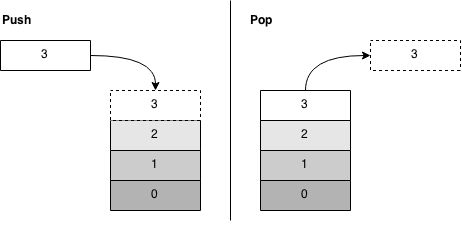
\includegraphics[scale=0.6]{images/stack.png}
  \caption{Stack push and pop operations}
  \label{fig:stack}
\end{figure}

% The stack was first introduced in 1946 by Alan Turing, while he was working on
% the Automatic Computing Engine (ACE)~\footnote{Automatic Computing Engine (ACE):
% \url{http://en.wikipedia.org/wiki/Automatic_Computing_Engine}} at the National
% Physical Laboratory (NPL)~\footnote{National Physical Laboratory:
% \url{http://en.wikipedia.org/wiki/National_Physical_Laboratory_(United_Kingdom)}}
% in the UK:
% \begin{quote}
%   [Alan Turing] outlined a method for leaving one line of work being carried out
%   on the computer, calling up a subsidiary line, and then returing to the first
%   line when finished with the subsidiary line. He called the calling up and
%   returning routines BURY and UNBURY.~(\textcite[82]{newton})
% \end{quote}
% Here, BURY and UNBURY are synonymous with push and pop.

% @book{newton,
% author    = "David E. Newton",
% year      = 2003,
% title     = "Alan Turing : a study in light and shadow",
% publisher = "[Philadelphia]: Xlibris",
% ISBN      = 9781401090791
% }

Although, essentially, one cannot take the second element from top without first
removing the top most element, the model can easily be modified to support such
operations. For instance, a common stack operation is {\it peek}, which reads
the value of the top element without actually removing it. This can easily be
done by popping, storing the value and pushing it back to the stack. Other
operations can be implemented in a similar fashion.

\subsubsection{Stack vs. Register Machine}
Machines can implement the stack model virtually and execute it directly in
hardware, but as we are designing an abstract machine, we will only discuss the
virtual aspect. Regardless, such a machine is commonly called a \term{stack
  machine}.

The most common notation in arithmetic formulas and statements are the infix
notation, where the operator is written between its operands: $1 + 2$. One can
express the same statement with prefix notation, also called \term{Polish
  notation}: $+\ 1\ 2$. When programming stack machines, one uses what is called
the \term{reverse Polish notation}, which is in fact postfix notation:
$1\ 2\ +$. By using this notation, one can easily convert this into stack
operations, where $1\ 2\ +$ becomes:
\begin{stackops}
  \op{push 1}{1}
  \op{push 2}{2,\ 1}
  \op{add}{3}
\end{stackops}

Here the {\tt add} operation pops two elements, adds them together and pushes
the result back onto the stack.

As briefly discussed in the~\ref{sec:background} section, a register machine
TODO

\subsubsection{Stack Organization}
% All stacks will initially have a single activation frame

The stacks will not be limited in size, as the stacks can be implemented as heap
object which can grow dynamically. Through out this report, we will say that the
stacks \term{grows downwards}. This is because physically, the top most element
of the stack is located at a low address in the host computers
memory. Therefore, as more elements are pushed to the stack, they will get
higher addresses, making the stack grow downwards in memory.

A stack element will consist of some type information and a reference to its
content, or data. The type information will include its declared type, but also
an actual type. For statically typed languages, these will most likely (TODO: ?)
be the same. For dynamic languages this is required to hold track of an
element's type, as its allowed to assign a value type an element, which was
originally declared with an other type.

\subsubsection{Stack Manipulation}
As mentioned above, there will we instructions for doing simple stack
manipulations, for instance {\tt push} and {\tt pop}. As we will see later,
these two instructions alone will be very limiting, and make the job of writing
a compiler very tedious. Therefor, we will need more instructions, making more
complex manipulations more convenient.

When we later describe the execution model of the machine, we will see that we
need instructions for pushing an popping elements further up the stack. For
instance, if we want to access the arguments given to a subroutine, they will be
located up the stack. The compiler will therefor need an effective method of
duplicating that element onto the top of the stack, making is accessible for
further computation. Also it will need to push an element to a specific position
up the stack, effectively returning a value to the caller.

Such versions of the push and pop operations will take an displacement argument,
saying how many places up the stack it is to push to or pop from. To make this
as convenient as possible, the displacement will be from the top of the stack,
meaning displacement 0 will be the top of the stack. Exception handling will
have to be utilized when using a displacement which is not allowed, for instance
outside the stack or its own scope.

Lets call these two instructions {\tt pushElement} and {\tt
  storeElement}. Unlike {\tt push}, which adds a new element to the stack, the
specification defines {\tt pushElement} to overwrite the element at the given
displacement. This is more convenient as this does not change the displacement
of the following elements, though it requires some planning, as there will have
to be an element on the stack with the purpose of being overwritten. {\tt
  storeElement} will pop of the top-most element and place it at the given
displacement.

Also, unlike our previous stack example, the {\tt push} instruction, or rather
the {\tt pushElement} instruction, will not take a value as an argument. Rather
it will take the element at the given displacement and push onto the top of the
stack. There will be separate instructions for adding new elements onto the
stack, for instance {\tt pushConstant}.

Here we can see some simple operations using the {\tt pushElement} and {\tt
  popElement} operations.
\begin{stackops}
  \op{-}{3,\ 1,\ 1}
  \op{pushElement 0}{3,\ 1,\ 1,\ 3}
\end{stackops}


\subsection{Threading}
\label{sec:design:threading}
Big chip manufacturers like Intel, have always been under big pressure to
deliver ever faster processors, year after year. For around the last decade, the
technological development of processors has been focused adding cores rather
than increasing the clock speed, which already started to stagnate around
2004~\cite{sutter}. With multiple processors, or popularly called a multi-core
processor, processes may actually run in parallel, i.e. running at the same
time, rather than just concurrently where multiple processes actually share the
same processor.

A thread is typically the smallest unit of executable instructions by a
processor. A process being run by an operating system therefore had one thread
which the operating systems scheduler delegated CPU time to. With multi-core
processors, the notion of a single process having multiple threads arose, making

Although multi-threading is a very interesting feature, it also raises a lot of
challenges when designing machines. Different threads cannot directly read and
write to the same place, or address, in memory without taking data races into
account, which is a common mistake when writing multi-threaded programs. If
multiple threads are reading and writing to the same memory, it is impossible
for the threads to base any logic on it, as another thread can change its value
at any time, effectively pulling the rug from under you. This problem as been
named the mutual exclusion problem, and is solved by using synchronization
structures.

Our machine will both support threading and synchronization structures
therefor. As we are using a stack machine, each thread has to have its own
state, including its own stack. In other words, all stacks are private and
cannot be shared across threads. This can though be facilitated by using heap
object which are referenced from multiple threads' stack.

\subsubsection{Tasks and Transactions}
TODO
% Multiple executables may execute simultaneously.
% Task and transaction semantics is supported. A transaction is considered
% executed by the thread starting it. A spawned task is independent of the spawn-
% ing thread and may be executed by the spawning thread or some other thread.
% However, tasks will not migrate between threads so the thread which started
% execution of a task will also complete the task.

% Tasks do not share stacks with the spawning thread, spawning task, or any
% other task. Implementations may, however, execute tasks using the stack of the
% executing thread. The executed task is not allowed to access any stack space
% beyond its initial set of stack elements. The implementation must throw an
% exception if any such offending access is attempted.

\subsubsection{Thread Pool}
Creating and destroying system threads is not free. If a new thread is created
on demand, it would create significant overhead. Another problem with this model
is the risk of resource thrashing. If there is no limit on the number of threads
that can be created, it can intentionally or unintentionally be exposed to heavy
abuse. A solution to both of these challenges is having what is called a
\term{thread pool}. On machine initialization, a set number of threads is
pre-initialized and stored in a data structure. When a thread tries to spawn a
new thread, it is given one from the thread pool. If the thread pool is empty,
it has to wait for a thread to become vacant.

This model, although effective, also brings with it some
challenges. Specifically, when the thread pool is empty. The spawning thread
cannot stop and wait until a new thread is vacant, as this would block the whole
thread. Rather, the machine will use a work queue. A work queue manages the
thread pool so other threads does not need to wait for a thread to become
vacant, and thereafter fight with each other of whom gets to take it. The
spawning threads would give the task which it wants run in a new thread, to the
work queue. The queue would monitor the thread pool and as soon as a thread
becomes free, it would take the task first in the work queue and run in.

\subsubsection{Errors and Exceptions}
Two types of errors can occur; internal errors in the machine and errors
produced by the program the machine is executing. Internal errors will most
likely occur in some child thread and not in the process' original thread. If
that is the case we would stop that thread and gracefully stop the machine if it
cannot safely continue. If the error occurs in the process' original thread, we
will in most cases still be able to catch the signal sent by the OS and
gracefully stop.

When the program being executed produces an \term{exception} it will percolate
up through a defined set of exception handlers until it is handled. If there is
no way of handling the exception it called an uncaught exception. It that case
the machine will print some information on the exception and stop. It will not
attempt to join all threads (TODO) as it cannot know how long this will
take. Therefore all threads are exited and memory is freed, ensuring no memory
leaks.

TODO: Exception handling


\subsection{Types}

The type system of \thename{} aims to enable efficient implementation of both
dynamically and statically typed languages. That gives rise to a need for an
adaptable system that is capable of describing arbitrarily complex types along
with potential storage layout information for languages that require explicit
memory layout of objects. Moreover the system must be flexible and modifiable
during run-time, e.g.~to allow dynamic languages to add and remove members of an
object while still being able to properly type check the code.

\subsubsection{DWARF}

Types are expressed in the DWARF format\cite{dwarf}. DWARF is a format mainly
used to describe debug information for executable files, essentially by
describing the source code of a program and mappings into to the compiled
binary. It is used in many modern compilers\footnote{Usages include GCC, Clang
  and Go} and is commonly used in combination with ELF binaries. It provides a
method to describe everything from source code locations, scopes, exception
handling, compilation units, linking information, etc. The primary building
block of DWARF information is the Debug Information Entry (DIE). It consists of
a DWARF tag that describes the kind of entry, and a set of attributes that
further defines the characteristics of an entry. Tags and attributes can be
nested which enables types to be as intricate as necessary. It is worth to
mention that DWARF is simply a \emph{format}, and while there are libraries to
help read and write the format, they are not part of the DWARF specification.

We do not use the full set of features provided by DWARF, rather we only use
DIEs for type information in ELF files. We would most likely also use DWARF to
facilitate proper debugging, but that is beyond the scope of this thesis.

DWARF DIEs are tree structures and we will use indention based notation to
present them. Listing~\ref{lst:design:dwarf:basic} shows how we can use DWARF to
express a 32-bit signed integer. Note that the name ``int'' has no special
meaning in DWARF, but consumers of DWARF may put special meaning into names.

\begin{lstlisting}[
  caption={A simple DWARF DIE describing a 32-bit signed integer},
  label={lst:design:dwarf:basic}]
<1> DW_TAG_base_type
        DW_AT_name = int
        DW_AT_byte_size = 4
        DW_AT_encoding = signed
\end{lstlisting}

In the above, there is a single tag with three attributes that describe the
type's name, size and encoding. The \code{DW\_TAG\_base\_type} essentially
designates a primitive type, one that is not a compound of one or more types,
and will usually be a leaf in the DWARF tree. For types that \emph{are}
compound, the approach is to store DIEs in an indexed table and reference types
by their index location in the table. In the above, the type's index is
designated by the \code{<1>}. By doing this no type ever has to be duplicated,
because any other types simply reference the same index. Tags start with the
\code{DW\_TAG\_} prefix while attributes use \code{DW\_AT\_}, all of which are
simply names for integer constants defined by the DWARF specification.

Listing~\ref{lst:design:dwarf:complex} shows a more complex example with a
subprogram (i.e.~a subroutine) that returns a pointer to the integer type
defined above.

\begin{lstlisting}[
  caption={A more complex example of DWARF types referencing each other},
  label={lst:design:dwarf:complex}]
<2> DW_TAG_pointer_type
        DW_AT_byte_size = 4
        DW_AT_type = <1>

<3> DW_TAG_subprogram
        DW_AT_name = foo
        DW_AT_type = <2>
        DW_AT_low_pc = 0x1
        DW_AT_high_pc = 0x10
\end{lstlisting}

It is shown how type \code{<2>} is defined as a pointer to the type \code{<1>},
which in C lingo is \code{int*}. Type \code{<3>} defines a subroutine whose name
is ``foo'' and returns a \code{<2>}, again in C lingo that would be \code{int
  *foo()}. This is the fundamental way that the DWARF format expresses types; it
is simple but very flexible and powerful.

There are scores of attributes and tags defined in the specification, but we do
not nearly use all of them. Because the format is so simple it is easy to add
new tags and attributes, simply by defining a new tag or attribute and a
corresponding numeric constant and documenting it. \thename{} defines some tags
TODO.

DWARF DIEs are, as mentioned, tree structures which is effective for expressing
types but is not very compact for storage,and can result in potentially unwieldy
data. There are more than one way to store the tree structure in a compact
manner, one of which we will describe here. TODO (which one does bfd use?).

\subsubsection{\thename{}'s Types System}

\thename{} provides a set of built-in types, encompassing both primitive types
as well as references, arrays and composite types. Further there is the concept
of a meta kinds which essentially wraps type definitions, type references,
subroutines, etc.~into a unified meta-data kind which are all stored in a single
table in the executable.

Compilers can map their primitive types to the ones provided by \thename{}, and
we expect that combinations of the available compound types to be sufficient for
expressing any other conceivable type however complex.

Below is a description of the various kinds of simple types provided.

\begin{description}
\item[Integer values] \hfill\\
  Includes all combinations of 8-bit, 16-bit and 32-bit, signed or unsigned
  integer numbers. E.g. {\tt Int32} and {\tt UInt16}.

\item[Boolean] \hfill\\
  A {\tt Boolean} type with the values `true` or `false`.

\item[Floating point values] \hfill\\
  32-bit or 64-bit floating point numbers, in the IEEE 753-1985 or IEEE 755-1985
  standard representation, respectively named {\tt Ieee32} and {\tt Ieee64}.

\item[Address] \hfill\\
  Unsigned integer value representing a memory address, named {\tt
    Address}. This is considered unsafe, and will therefore only be possible in
  code declared as `unsafe`.

\item[Abstract] \hfill\\
  Type which can take any value at run-time, named {\tt AnyType}. Large values
  will be boxed on the heap to make space for it.
\end{description}

% reference

The machine has a set of reference types, with the most fundamental being the
{\tt Reference <t>} type. This allows heap objects to be referenced from the
stack. As the name suggests, it will take a type of the object it referenced as
argument. In the opposite scenario, there is a {\tt StackReference <t>} type,
allowing passing references directly to stack references. This type may not be
boxed, nor passed to threaded tasks. This will save programs from major pitfalls
in concurrent programs (?).

To support variable argument calling conventions, letting a subroutine take an
arbitrary number of arguments, a special reference type is needed. This is done
through an {\tt ArgumentReference}, allowing a subroutine to iterate over its
given arguments. Also, to referencing a subroutine will be done through a {\tt
  CodeReference <signature>}, taking the signature which it implements. This is
a meta type, described below.

% arrays

The machine supports two types of arrays; a static and a dynamic type. Both will
be generic, taking the type of its values. This could be to other arrays,
allowing an array to be multi-dimensional. The static variant will also take a
lower and higher limit of values, aptly named {\tt StaticArray
  <t><lowerLimit><higherLimit>}. The dynamic variant will not take the limits,
as therefore named {\tt DynamicArray <t>}. To allow it to grow dynamically, it
will be instanced and put on the heap. It will therefore be referenced through a
{\tt Reference} type.

% composite

To support custom types, similar to a struct in the C programming language,
there will be a {\tt Composite <t+>} type. This will take an arbitrary number of
type arguments, describing its member. Though not visible from the type
signature, each member will have a name, allowing for convenient referencing (TODO).

Lastly, the machine will have a set of meta types, describing types by them
selves. These include {\tt Type}, {\tt Signature} and {\tt TypeSignature}. (TODO)


% Examples of how to map things to our model ()
%% Classes
%% Inheritance
%% HoF
%% Polymorphism

% Type system
%% Representation (DWARF)
%% Typed instructions
%% Run-time type checking
%% Dynamic types
%%% !!!

% Executable format
%% ELF
%%% It's tried-and-true
%%% Everybody else uses it so we can port stuff easier

% Object model
%% Virtual tables
%% Hash maps
%%% The efficiency of them
%% Dynamic dispatches

% Threading
%% Tasks and transactions
%%% Shared stack elements
%% ?!
%% Thread Pool
%%% Resource thrashin

% Closures

% Memory management
%% Garbage collection

% ISA
%% Highlight the most important instructions, explain how they facilitate the above


% Mem model
%% Standard heap and stack, stack per thread, global heap
%%

%%% Local Variables:
%%% mode: latex
%%% TeX-master: "../report"
%%% End:
